\newpage

\hypertarget{annexe}{%
\section{Annexe}\label{annexe}}

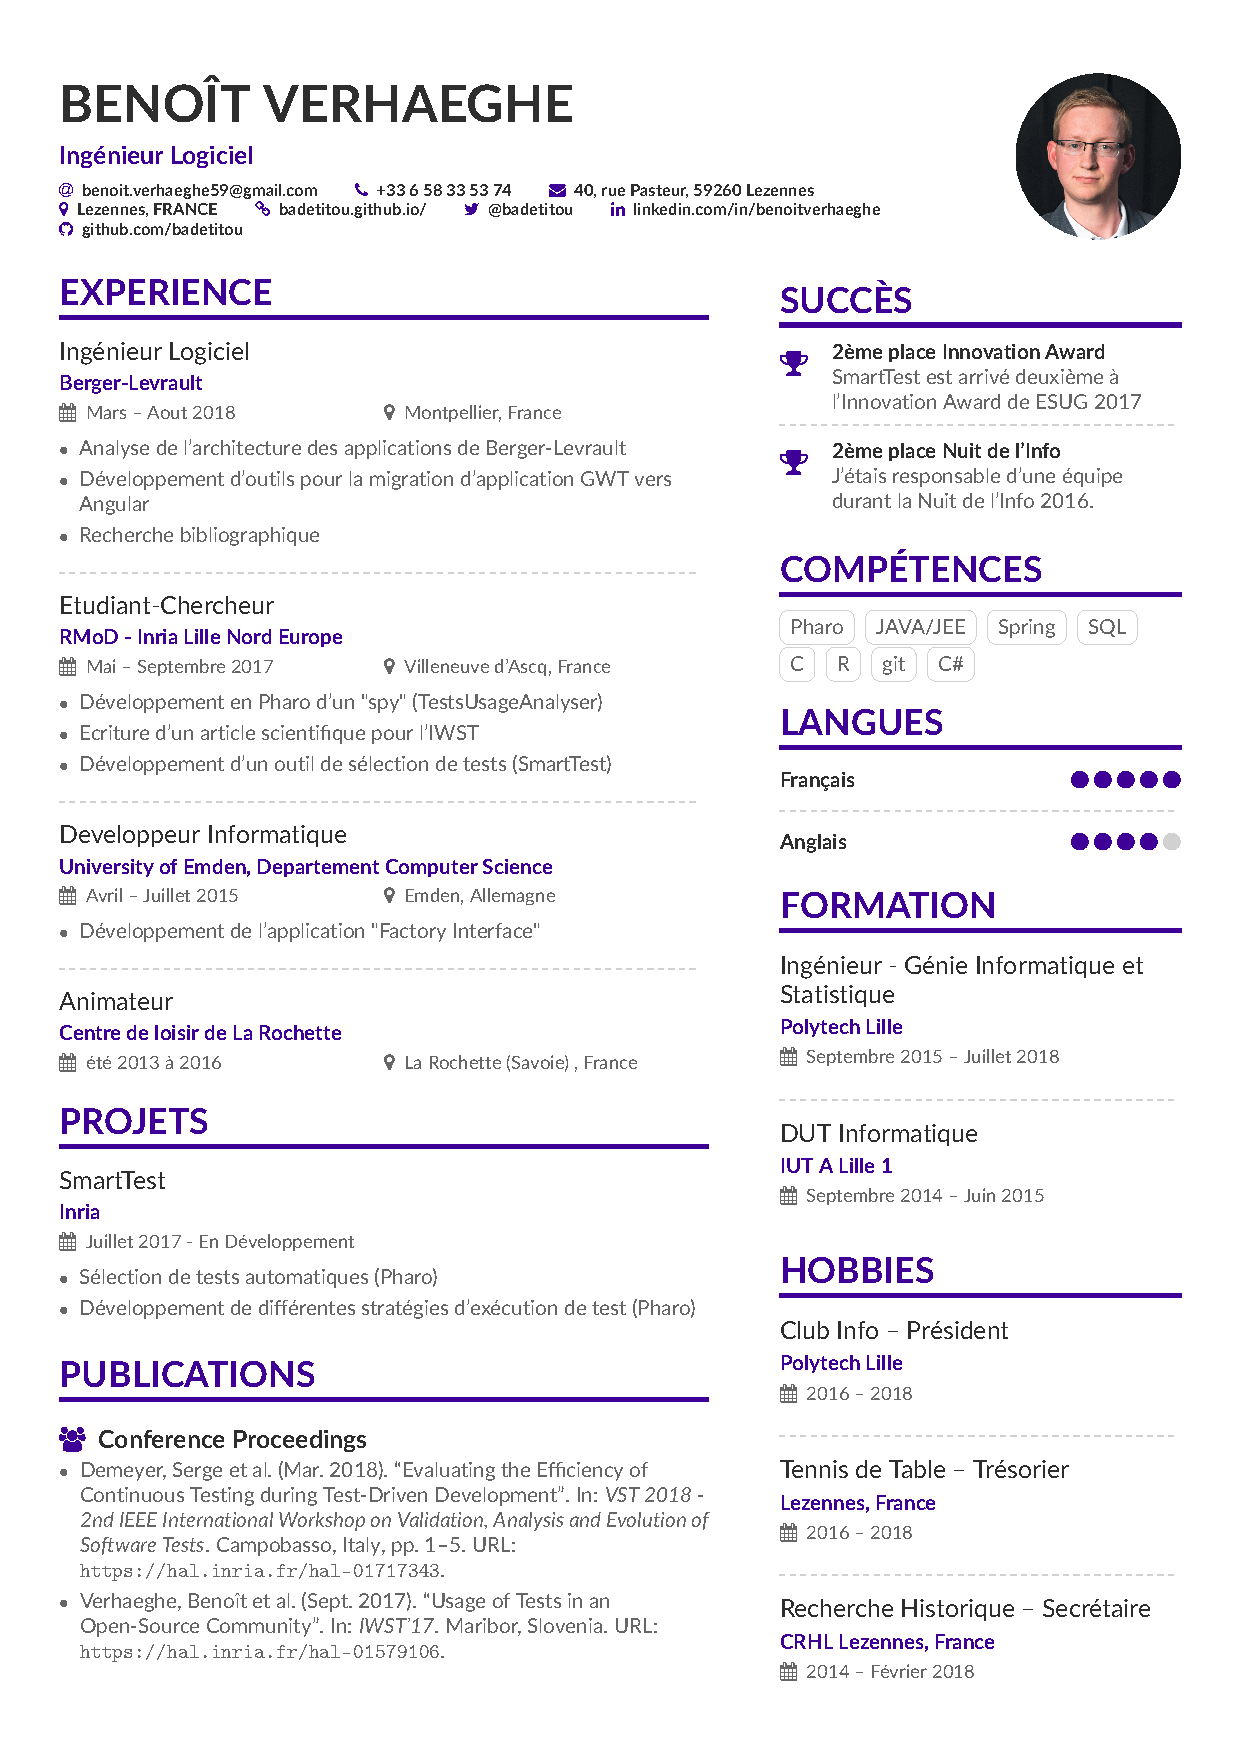
\includegraphics[width=0.9\textwidth,height=\textheight]{cv/cv.pdf}
\newpage

\hypertarget{ruxe9sumuxe9}{%
\section*{Résumé}\label{ruxe9sumuxe9}}
\addcontentsline{toc}{section}{Résumé}

\hypertarget{franuxe7ais}{%
\subsection*{Français}\label{franuxe7ais}}
\addcontentsline{toc}{subsection}{Français}

Berger-Levrault est une entreprise majeur dans le monde de l'édition de
logiciel. Dans le cadre de l'évolution de ses applications, elle
souhaite changer le langage d'implémentation de ces derniers. Pour cela,
un travail préliminaire a été mené en Projet de Fin d'Étude où l'on a
étudié une application de démonstration (« application
\emph{bac-à-sable} ») qui reprend les principes d'organisation des
applications de Berger-Levrault. Le but de ce stage est de vérifier que
les résultats de l'étude préalable réalisée durant le PFE peut être
appliqué grandeur nature sur des applications en production de
Berger-Levrault et définir et implémenter une stratégie pour effectuer
la migration des applications. Lors de ce projet, nous avons notamment ;

\begin{itemize}
\tightlist
\item
  Modélisé des interfaces graphique d'applications client de
  Berger-Levrault. Le but de cette modélisation est de fournir le
  maximum d'information sur les écran de l'application pour permettre
  une ré-implémentation (semi-)automatique dans une autre langage ;
\item
  Extrait automatique des composants des différents écrans de
  l'application;
\item
  Extrait d'une carte de navigation entre ces écrans (quel écran permet
  de passer à quel autre écran) ;
\item
  Définit une stratégie, passant par l'utilisation de modèles, pour
  effectuer la migration d'une application disposant d'une interface
  graphique
\item
  Réalisé un état de l'art sur le domaine de la migration d'application.
\item
  Migré l'application \emph{bac-à-sable} de GWT vers Angular.
\end{itemize}

\hypertarget{anglais}{%
\subsection*{Anglais}\label{anglais}}
\addcontentsline{toc}{subsection}{Anglais}
